\section{Endcap Muon System Upgrade}
\label{sec:csc_upgrade}

All CSCs in ME4/2 rings have been installed during LS1. This results in four measurement stations for muons in the region $1.25 < |\eta| < 1.8$ providing additional redundancy in a high rate environment. This redundancy is especially important for future upgraded Global Muon Trigger (GMT) algorithms. For the CSC Track Finder (TF) additional measurement in this region will increase the efficiency and improve the rate reduction since it will be more likely to have 3 or more hits used in the $p_T$ assignment logic. No additional hardware or reconfiguration of the present muon trigger was required after this upgrade. The muon sector receiver boards for the fourth disk already were in place and the present CSCTF already had logic to process trigger data from these chambers.

Electronics for the CSCs have been also under major revision during LS1. All CSCs in ME1/1 rings received new digital cathode front-end boards (DCFEB) as well as new optical trigger motherboards (OTMB) and optical data acquisition motherboars (ODMB) as schematically shown in Fig.~\ref{fig:me11_upgrade_overview}. The new electronics will significantly enhance ME1/1 performance in the trigger and in the offline reconstruction providing a key sagitta measurement for the muon L1 trigger in the region $1.6 < |\eta| < 2.4$. The recovered old electronic boards were used to instrument the newly installed ME4/2 chambers.

The strips of the ME1/1 chambers are split into two regions at $|\eta| = 2.1$ (see details on mechanical layout and signal readout of the ME1/1 chambers in Appendix~\ref{app:me11}). The bottom region ($2.1 < |\eta| < 2.4$) previously had 48 strips triple-ganged to 16 channels in the electronics for both the trigger and the readout, making hit recognition ambiguous. The ambiguity can be mitigated using measurements from the outer stations. However, the $p_T$ resolution using only the outer stations is quite coarse, leading to a significantly increased single muon trigger rate in the forward region $2.1<|\eta|<2.4$. As a result, this region generated a single muon trigger rate comparable to that of the entire region $|\eta| < 2.1$. With the new seven DCFEBs per chamber, this triple-ganging is removed, leading to improved triggering performance in the forward region which allows to maintain highly efficient muon trigger coverage up to $|\eta| = 2.4$.

\begin{figure}[b]
        \begin{center}
                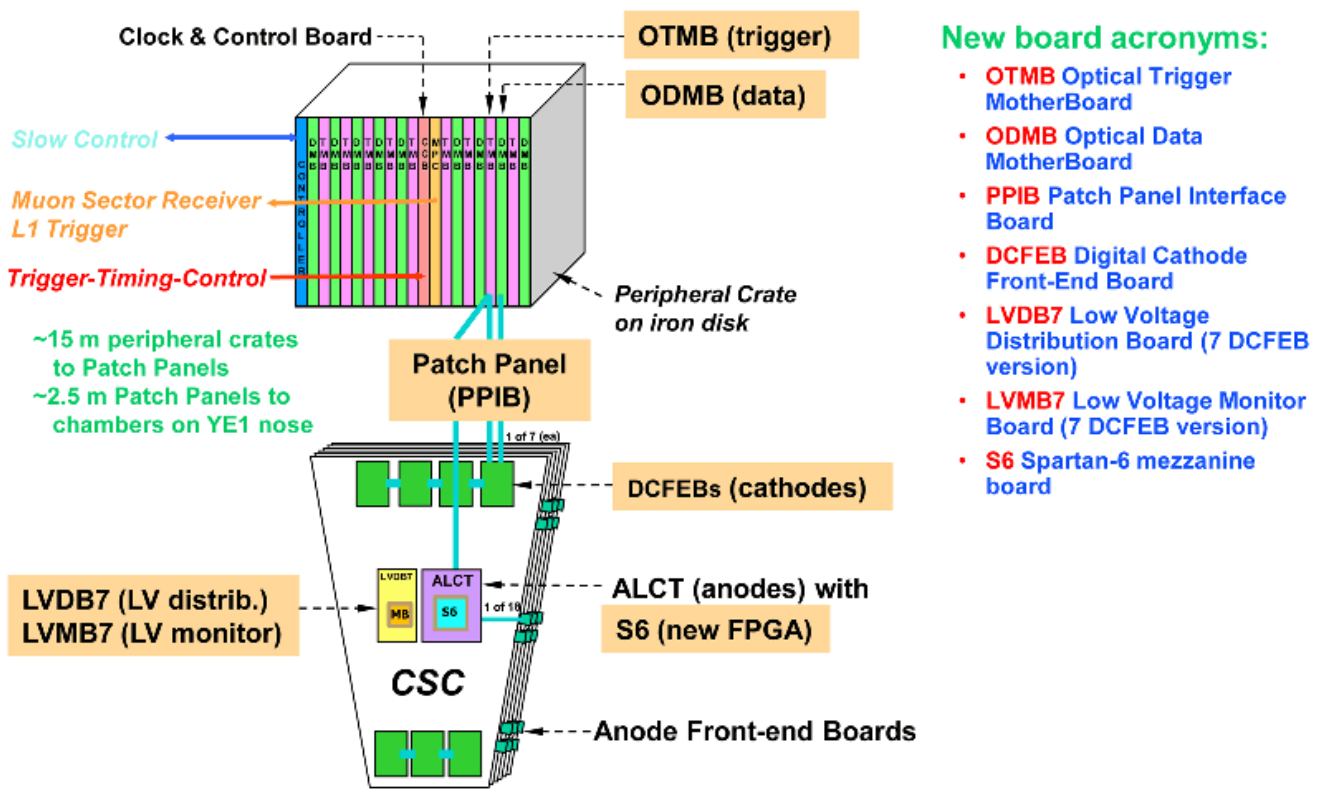
\includegraphics[width=0.85\linewidth]{figures/ME11_upgrade_overview.png}
                \caption{Schematic overview of the ME1/1 electronics upgrade after LS1.}
                \label{fig:me11_upgrade_overview}
        \end{center}
\end{figure}